\documentclass{article}

\usepackage{amsmath,amsfonts,amssymb,amsthm}
\usepackage{enumerate}
\usepackage{arydshln}
\usepackage{listings,color}
\usepackage{graphicx}

\definecolor{dkgreen}{rgb}{0,0.6,0}
\definecolor{gray}{rgb}{0.5,0.5,0.5}
\definecolor{mauve}{rgb}{0.58,0,0.82}

% Opening
\title{Numerical Analysis HW8\\
Ch12 - 3,9 (pg300)\\
Ch13 - 1,3 (pg317)\\}
\author{Neal D. Nesbitt}

\begin{document}
\maketitle

\theoremstyle{definition}
\newtheorem{problem}{Problem}
\newtheorem{solution}{Solution}[problem]

\lstset{basicstyle=\ttfamily,
		language=Matlab,
		keywordstyle=\color{blue},
		commentstyle=\color{dkgreen},
		stringstyle=\color{mauve},
		identifierstyle=\bf
		}

\setcounter{problem}{2}
\begin{problem}
Use the Gauss-Seidel method to solve the following system until the percent relative error falls below $\epsilon_{r}= 5\%$\\
\[
\begin{matrix}
10x_{1}	&+2x_{2}	&-x_{3}	&=	27\\
-3x_{1}	&-6x_{2}	&+2x_{3}	&=	-61.5\\
x_{1}	&+x_{2}	&+5x_{3}	&=	-21.5
\end{matrix}
\]
\end{problem}

\begin{solution}
If we use the iterative Gauss-Seidel method, then starting with a normalized right hand side for our initial guess, each iteration we use our current approximated terms to back-substitute the current line for the current term. If we keep track of each iteration as a full run through all the coordinate terms of the approximation, the results give:
\[
\begin{bmatrix}
2.7000\\
8.9000\\
-6.6200
\end{bmatrix}
\to
\begin{bmatrix}
0.2580\\
7.9143\\
-5.9345
\end{bmatrix}
\to
\begin{bmatrix}
0.5237\\
8.0100\\
-6.0067
\end{bmatrix}
\to
\begin{bmatrix}
0.4973\\
7.9991\\
-5.9993\\
\end{bmatrix}
\to
\begin{bmatrix}
0.5003\\
8.0001\\
-6.0001
\end{bmatrix}
\]
while the corresponding relative error for each iteration's terms is
\[
\begin{bmatrix}
100\\
100\\
100
\end{bmatrix}
\to
\begin{bmatrix}
946.5116\\
12.4542\\
11.5517
\end{bmatrix}
\to
\begin{bmatrix}
50.7339\\
1.1944\\
1.2032
\end{bmatrix}
\to
\begin{bmatrix}
5.3005\\
0.1364\\
0.1243
\end{bmatrix}
\to
\begin{bmatrix}
0.5852\\
0.0128\\
0.0132
\end{bmatrix}
\]
\end{solution}

\setcounter{problem}{8}
\begin{problem}
Determine the solutions of the simultaneous nonlinear equations:\\
\[ 
\begin{matrix}
x^{2} = 5-y^{2}\\
x^{2} = y+1
\end{matrix}
\]
\begin{enumerate}[(a)]
\item Graphically.
\item Successive substitution using initial guesses of $x=y=1.5$
\item Newton-Raphson using initial guesses of $x=y=1.5$
\end{enumerate}
\end{problem}

\begin{solution}
Graphically we can plot both curves with respect to x and y and visually estimate where they intersect:\\
\begin{align*}
x&=\sqrt{5-y^{2}}\\
y&=x^{2}-1
\end{align*}
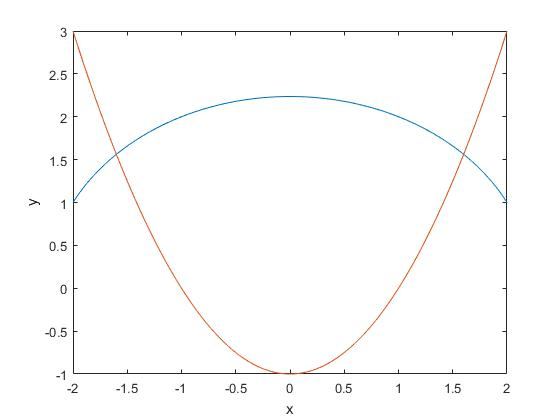
\includegraphics[width=\linewidth]{HW8-NonlinearGraph.jpg}
It appears that there are solutions at roughly $(x\approx\pm 1.5,y=1.5)$
\end{solution}

\begin{solution}
For successive substitution we have to pick a way to substitute in the values.
\begin{align*}
x&=\sqrt{5-y^{2}}	&	y&=\sqrt{5-x^{2}}\\
y&=x^{2}-1			&	x&=\sqrt{y+1}
\end{align*}
\paragraph{}
If we choose the left pair, and make the given initial guess we end up finding that the solutions don't converge.
\[
\begin{bmatrix}
x\\
y
\end{bmatrix}
=
\begin{bmatrix}
1.5\\
1.5
\end{bmatrix}
\to
\begin{bmatrix}
1.6583\\
1.7500
\end{bmatrix}
\to
\begin{bmatrix}
1.3919\\
0.9375
\end{bmatrix}
\to
\begin{bmatrix}
2.0300\\
3.1211
\end{bmatrix}
\]
But if we use the right set of equations we get
\[
\begin{bmatrix}
y\\
x
\end{bmatrix}
=
\begin{bmatrix}
1.5\\
1.5
\end{bmatrix}
\to
\begin{bmatrix}
1.6583\\
1.6304
\end{bmatrix}
\to
\begin{bmatrix}
1.5303\\
1.5907
\end{bmatrix}
\to
\begin{bmatrix}
1.5715\\
1.6036
\end{bmatrix}
\to
\begin{bmatrix}
1.5584\\
1.5995
\end{bmatrix}
\to
\begin{bmatrix}
1.5626\\
1.6008
\end{bmatrix}
\to
\begin{bmatrix}
1.5612\\
1.6004
\end{bmatrix}
\]
Which suggests this root approximation converges to $(y=1.562,x=1.600)$
\end{solution}

\begin{solution}
Using the Newton-Raphson method with the same initial guesses $(y=1.5,x=1.5)$ gives a wild solution that oscillates back and forth and moves away from the solution very rapidly.
\end{solution}

\setcounter{problem}{0}
\begin{problem}
Repeat example 13.1, but for three masses with the $m\text{'s}=40\text{ kg}$ and the $k\text{'s}=240\text{ N/m}$. Produce a plot like Fig. 13.4 to identify the principle modes of vibration.
\end{problem}

\begin{solution}
If we construct a mass and spring system as in Example 13.1 and 13.2, but in this case with 3 masses $m=40\text{ kg}$, and 4 springs with constants $k = 240\text{ N/m}$, we can develop a set of equations from the free body diagrams of each mass about its point of equilibrium. Let $a$ be the acceleration of each mass, $x$ be the position right of equilibrium on the track of each mass, and $F$ be the sum of net forces on each mass. Then
\begin{align*}
\begin{bmatrix}
F_{1}\\
F_{2}\\
F_{3}
\end{bmatrix}
&=
\begin{bmatrix}
m_{1}a_{1}\\
m_{2}a_{2}\\
m_{3}a_{3}
\end{bmatrix}
\\
\begin{bmatrix}
-kx_{1} +k(x_{2}-x_{1})\\
-k(x_{2}-x_{1})+k(x_{3}-x_{2})\\
-k(x_{3}-x_{2})-kx_{3}
\end{bmatrix}
&=
\begin{bmatrix}
m_{1}a_{1}\\
m_{2}a_{2}\\
m_{3}a_{3}
\end{bmatrix}
\\
k
\begin{bmatrix}
-2x_{1}+x_{2}\\
x_{1}-2x_{2}+x_{3}\\
x_{2}-2x_{3}
\end{bmatrix}
&=
\begin{bmatrix}
m_{1}a_{1}\\
m_{2}a_{2}\\
m_{3}a_{3}
\end{bmatrix}
\\
k
\begin{bmatrix}
-2	&	1	&	0\\
1	&	-2	&	1\\
0	&	1	&	-2
\end{bmatrix}
\begin{bmatrix}
x_{1}\\
x_{2}\\
x_{3}
\end{bmatrix}
&=
\begin{bmatrix}
m_{1}a_{1}\\
m_{2}a_{2}\\
m_{3}a_{3}
\end{bmatrix}
\end{align*}
We can then take this resulting matrix and find the characteristic polynomial
\[ 
\begin{vmatrix}
-2-\lambda	&	1	&	0\\
1	&	-2-\lambda	&	1\\
0	&	1	&	-2-\lambda
\end{vmatrix}
=  -(\lambda+2)^{3}+2(\lambda+2) 
= -(\lambda+2)((\lambda+2)^{2}-2) 
= -(\lambda+2)(\lambda^{2}+4\lambda+2)
\]
Thus there are three eigenvalues associated with the system:
\begin{align*}
\lambda_{1} &= \boxed{-2}\\
\lambda_{2} &= \frac{1}{2}(-4+\sqrt{16-8}) = \boxed{-2+\sqrt{2}}\\
\lambda_{2} &= \frac{1}{2}(-4-\sqrt{16-8}) = \boxed{-(2+\sqrt{2})}
\end{align*}
and then we can reconstruct our system and back solve
\[
\begin{bmatrix}
-2-\lambda	&	1	&	0\\
1	&	-2-\lambda	&	1\\
0	&	1	&	-2-\lambda
\end{bmatrix}
\begin{bmatrix}
x_{1}\\
x_{2}\\
x_{3}
\end{bmatrix}
= 0
\]
for each eigenvalue.

\paragraph{}
So for $\lambda=-2$
\begin{align*}
\begin{bmatrix}
-2-2	&	1	&	0\\
1	&	-2-2	&	1\\
0	&	1	&	-2-2
\end{bmatrix}
\begin{bmatrix}
x_{1}\\
x_{2}\\
x_{3}
\end{bmatrix}
&= 0\\
\begin{bmatrix}
-4	&	1	&	0\\
1	&	-4	&	1\\
0	&	1	&	-4
\end{bmatrix}
\begin{bmatrix}
x_{1}\\
x_{2}\\
x_{3}
\end{bmatrix}
&= 0
\end{align*}

\begin{align*}
&\begin{bmatrix}
-4	&	1	&	0\\
1	&	-4	&	1\\
0	&	1	&	-4
\end{bmatrix}
\to
\begin{bmatrix}
-4	&	1			&	0\\
0	&	-4-(1/4)	&	1\\
0	&	1			&	-4
\end{bmatrix}
\to
\begin{bmatrix}
-4	&	1		&	0\\
0	&	-(21/4)	&	1\\
0	&	1		&	-4
\end{bmatrix}
\\
&\to
\begin{bmatrix}
-4	&	1		&	0\\
0	&	-(21/4)	&	1\\
0	&	0		&	-4+(4/21)
\end{bmatrix}
\to
\begin{bmatrix}
-4	&	1		&	0\\
0	&	-(21/4)	&	1\\
0	&	0		&	-(80/21)
\end{bmatrix}
\end{align*}
Thus we can take $x_{3}$ to be a free variable, and back substitution gives
\begin{align*}
x_{2} &= (4/21)x_{3}\\
x_{1} &= x_{3}/21
\end{align*}

Thus for $\lambda=-2$, 
\[
\mathbf{x}_{\lambda} = x_{3}\begin{bmatrix}
1/21\\
4/21\\
1
\end{bmatrix}
\]

For the other eigenvalues $\lambda_{2},\lambda_{3} = -(2\pm\sqrt{2})$, the system reduces to
\begin{align*}
&\begin{bmatrix}
\pm\sqrt{2}	&	1			&	0\\
1			&	\pm\sqrt{2}	&	1\\
0			&	1			&	\pm\sqrt{2}
\end{bmatrix}
\to
\begin{bmatrix}
\pm\sqrt{2}	&	1			&	0\\
0			&	\pm\sqrt{2}-(1/\pm\sqrt{2})	&	1\\
0			&	1			&	\pm\sqrt{2}
\end{bmatrix}
\to
\begin{bmatrix}
\pm\sqrt{2}	&	1				&	0\\
0			&	\pm\sqrt{2}/2	&	1\\
0			&	1				&	\pm\sqrt{2}
\end{bmatrix}
\\
&\to
\begin{bmatrix}
\pm\sqrt{2}	&	1				&	0\\
0			&	\pm\sqrt{2}/2	&	1\\
0			&	0				&	\pm\sqrt{2}-(2/\pm\sqrt{2})
\end{bmatrix}
\to
\begin{bmatrix}
\pm\sqrt{2}	&	1				&	0\\
0			&	\pm\sqrt{2}/2	&	1\\
0			&	0				&	0
\end{bmatrix}
\end{align*}
Thus again $x_{3}$ is a free variable and we have
\begin{align*}
x_{2} &= \mp\sqrt{2}x_{3}\\
x_{1} &= x_{3}
\end{align*}
giving our last two eigenvectors
\[
\mathbf{x} = x_{3}
\begin{bmatrix}
1\\
\mp\sqrt{2}\\
1
\end{bmatrix}
=x_{3}
\begin{bmatrix}
1\\
-\sqrt{2}\\
1
\end{bmatrix}
,x_{3}
\begin{bmatrix}
1\\
\sqrt{2}\\
1
\end{bmatrix}
\]

All together then, the eigenvalue and eigenvector matrices are
\[ 
\begin{bmatrix}
\lambda_{1}\\
\lambda_{2}\\
\lambda_{3}
\end{bmatrix}
=
\begin{bmatrix}
-2\\
-2+\sqrt{2}\\
-2-\sqrt{2}
\end{bmatrix},
\begin{bmatrix}
\mathbf{x}_{\lambda_{1}}	&	\mathbf{x}_{\lambda_{2}}	&	\mathbf{x}_{\lambda_{3}}
\end{bmatrix}
=
\begin{bmatrix}
1/21	&	1			&	1\\
4/21	&	-\sqrt{2}	&	\sqrt{2}\\
1		&	1			&	1
\end{bmatrix}
\]

Then we can look at the solutions of our original equation
\[ k
\begin{bmatrix}
-2	&	1	&	0\\
1	&	-2	&	1\\
0	&	1	&	-2
\end{bmatrix}
\begin{bmatrix}
x_{1}\\
x_{2}\\
x_{3}
\end{bmatrix}
=
\begin{bmatrix}
m_{1}a_{1}\\
m_{2}a_{2}\\
m_{3}a_{3}
\end{bmatrix} 
=
\begin{bmatrix}
m_{1}\\
m_{2}\\
m_{3}
\end{bmatrix}
\cdot
\begin{bmatrix}
d^{2}x_{1}/dt^{2}\\
d^{2}x_{2}/dt^{2}\\
d^{2}x_{3}/dt^{2}
\end{bmatrix}
\]

The physical explanation for this is again the modes of vibration for the system. Since we can assume that the general solutions for the positions of the masses are going to be superpositions of basic waveforms, then the first eigenvector represents the mode where all 3 masses are oscillating with the same frequency, but at different amplitudes. The second 2 eigenvectors also represent a system where the first and third mass move in tandem, but at the same amplitude. In these modes though, the mass in the middle moves farther, and while it moves at the same frequency, it can oscillate either in the same or in the opposite direction as the outer masses.

The superposition of these modes allows for a variety of seemingly chaotic resolutions of the system, all depending on the initial conditions.
\end{solution}

\setcounter{problem}{2}
\begin{problem}
Use the power method to determine the lowest eigenvalue and corresponding eigenvector for the system
\[
\begin{bmatrix}
2-\lambda	&	8			&	10			\\
8			&	4-\lambda	&	5			\\
10			&	5			&	7-\lambda
\end{bmatrix}
\]
\end{problem}

\end{document}